94. \begin{figure}[ht!]
\center{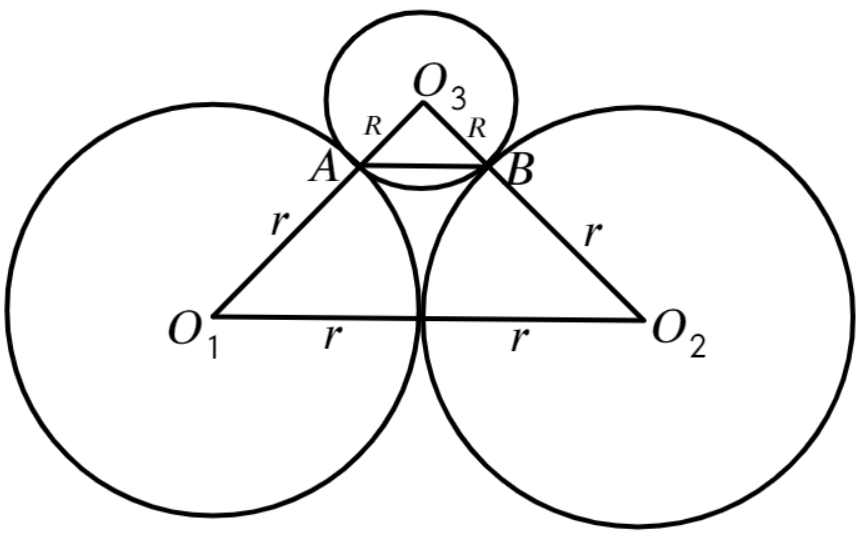
\includegraphics[scale=0.35]{g9-94.png}}
\end{figure}\\
Так как точки касания окружностей лежат на одной прямой с их центрами, имеем $O_1O_2=2r,$\\$O_1O_3=O_2O_3=R+r.$ Треугольники $O_1O_3O_2$ и $AO_3B$ подобны по двум сторонам и углу между ними (угол $O_3$ общий, $\cfrac{O_1O_3}{AO_3}=\cfrac{R+r}{R}=\cfrac{O_2O_3}{BO_3}),$ значит $\cfrac{2r}{12}=\cfrac{r+8}{8},\ 8r=6r+48,\ r=24.$\\
